\documentclass[10.5pt]{article}

\usepackage{graphicx}
\usepackage{multirow}
\usepackage{booktabs}
\usepackage{float}
\usepackage{setspace}
\usepackage{caption}
\usepackage{amsmath}
\usepackage{geometry}
\usepackage{lineno}
\usepackage{enumitem}

% bibliography/citations
\usepackage[super, comma, sort&compress]{natbib}

% hyperlinks should usually come after citation packages
\usepackage[colorlinks=true,linkcolor=black,citecolor=black,urlcolor=black]{hyperref}


\captionsetup[figure]{name=Figure,labelsep=period}
\captionsetup[table]{name=Table,labelsep=period}
\captionsetup{justification=centering}

\doublespacing
\setlength{\parindent}{0pt}

% Spacing Rules 

% Compact equation spacing
\setlength{\abovedisplayskip}{6pt}
\setlength{\belowdisplayskip}{4pt}
\setlength{\abovedisplayshortskip}{4pt}
\setlength{\belowdisplayshortskip}{4pt}

% Compact subsubsection spacing
\usepackage{titlesec}
\titlespacing*{\subsubsection}{0pt}{8pt}{4pt}




\usepackage{tocloft}

% Compact table of contents spacing
\setlength{\cftbeforesecskip}{0.15em}
\setlength{\cftbeforesubsecskip}{0.05em}
\setlength{\cftbeforesubsubsecskip}{0em}

% Slightly smaller TOC font
\renewcommand{\cftsecfont}{\small\bfseries}
\renewcommand{\cftsubsecfont}{\small}
\renewcommand{\cftsubsubsecfont}{\small}

\renewcommand{\cftsecpagefont}{\small\bfseries}
\renewcommand{\cftsubsecpagefont}{\small}
\renewcommand{\cftsubsubsecpagefont}{\small}



\usepackage{float} % put this in the preamble

\geometry{
    left=2.54cm,
    right=2.54cm,
    top=2cm,
    bottom=2.54cm
}

% \begin{figure}
%     \centering
%     \hspace*{1.7cm} % positive = shift right, negative = shift left
%     
\includegraphics[width=0.75\textwidth]{Screenshot_2026-04-29_at_11.48.08_PM.png}
% \end{figure}


\title{Preliminary Hemodialysis Membrane Design}


\author{
Aymen Ahmad, Kashfy Gazi, Radi Imran, Gabriel Pin de Jesus\\[0.5em]
\small Department of Chemical and Biological Engineering, University at Buffalo,\\
\small The State University of New York, Buffalo, New York, 14260-4200, USA.
}


\date{}






% \maketitle

\begin{document}

\begin{figure}[h]
    \centering
    
\includegraphics[width=0.75\textwidth]{Screenshot_2026-04-29_at_11.48.08_PM.png}
\end{figure}

\vspace{1.5cm}

\begin{center}
    {\LARGE Preliminary Hemodialysis Membrane Design\par}

    \vspace{0.35cm}

    {\large CE 318: Heat and Mass Transfer\par}

    \vspace{0.15cm}

    {\large Dr. Dave (Hsinhan) Tsai, PhD\par}

    \vspace{0.8cm}

    {\large Aymen Ahmad, Kashfy Gazi, Radi Imran, Gabriel Pin de Jesus\par}

    \vspace{0.5cm}

    {\small Department of Chemical and Biological Engineering, University at Buffalo,\par}

    \vspace{0.15cm}

    {\small The State University of New York, Buffalo, New York, 14260-4200, USA.\par}
\end{center}

\newpage

\tableofcontents

\newpage

\vspace{-1cm}


\clearpage





\subsection*{Nomenclature}

\vspace{-0.3cm}
\begin{description}
    \setlength\itemsep{-0.12cm}

    \item[\(A_m\)] Required membrane surface area, \(\mathrm{m^2}\).
    \item[\(C_A\)] Urea concentration, \(\mathrm{mg/L}\), \(\mathrm{kg/m^3}\), or \(\mathrm{mol/m^3}\).
    \item[\(C_{A,b}\)] Urea concentration on the blood side of the membrane.
    \item[\(C_{A,d}\)] Urea concentration on the dialysate side of the membrane.
    \item[\(C_{A,\mathrm{free}}\)] Free urea concentration available for diffusion.
    \item[\(C_{b,i}\)] Blood urea concentration entering the dialyzer.
    \item[\(C_{b,o}\)] Blood urea concentration leaving the dialyzer.
    \item[\(C_{d,i}\)] Dialysate urea concentration entering the dialyzer.
    \item[\(C_{d,o}\)] Dialysate urea concentration leaving the dialyzer.
    \item[\(C_{\mathrm{protein}}\)] Protein concentration in plasma, \(\mathrm{g/L}\) or \(\mathrm{kg/m^3}\).

    \item[\(D_{AB}\)] Molecular diffusivity of urea in water, \(\mathrm{m^2/s}\).
    \item[\(D_{AB,T}\)] Temperature-corrected urea diffusivity, \(\mathrm{m^2/s}\).
    \item[\(D_{AB,\mathrm{ref}}\)] Reference urea diffusivity, \(\mathrm{m^2/s}\).
    \item[\(D_{Ae}\)] Effective diffusivity of urea through the membrane, \(\mathrm{m^2/s}\).

    \item[\(d_f\)] Hollow fiber diameter, \(\mathrm{m}\).
    \item[\(f_{\mathrm{free}}\)] Fraction of urea available for diffusion.
    \item[\(J_A\)] Urea molar flux through the membrane, \(\mathrm{mol/(m^2 \cdot s)}\).
    \item[\(K_o\)] Overall mass-transfer coefficient, \(\mathrm{m/s}\).
    \item[\(k_b\)] Blood-side mass-transfer coefficient, \(\mathrm{m/s}\).
    \item[\(k_d\)] Dialysate-side mass-transfer coefficient, \(\mathrm{m/s}\).
    \item[\(L\)] Hollow fiber length, \(\mathrm{m}\).
    \item[\(\dot{m}_A\)] Mass rate of urea removal, \(\mathrm{mg/min}\) or \(\mathrm{kg/s}\).
    \item[\(\dot{n}_A\)] Molar rate of urea removal, \(\mathrm{mol/s}\).
    \item[\(MW_{\mathrm{protein}}\)] Average molecular weight of protein.
    \item[\(N_f\)] Number of hollow fibers.
    \item[\(Q_b\)] Blood volumetric flow rate, \(\mathrm{m^3/s}\), \(\mathrm{mL/min}\), or \(\mathrm{L/min}\).
    \item[\(Q_d\)] Dialysate volumetric flow rate, \(\mathrm{m^3/s}\), \(\mathrm{mL/min}\), or \(\mathrm{L/min}\).

    \item[\(T\)] Operating temperature, \(\mathrm{K}\) or \({^\circ}\mathrm{C}\).
    \item[\(T_{\mathrm{ref}}\)] Reference temperature, \(\mathrm{K}\) or \({^\circ}\mathrm{C}\).
    \item[\(v_b\)] Blood linear velocity, \(\mathrm{m/s}\).
    \item[\(v_d\)] Dialysate linear velocity, \(\mathrm{m/s}\).

    \item[\(\Delta C_1\)] Concentration difference at one end of the counter-current dialyzer.
    \item[\(\Delta C_2\)] Concentration difference at the opposite end of the counter-current dialyzer.
    \item[\(\Delta C_{lm}\)] Log-mean concentration difference, \(\mathrm{mg/L}\) or \(\mathrm{kg/m^3}\).

    \item[\(\delta_m\)] Membrane thickness, \(\mathrm{m}\).
    \item[\(\varepsilon\)] Membrane void fraction/porosity.
    \item[\(\mu_b\)] Blood viscosity, \(\mathrm{Pa \cdot s}\) or \(\mathrm{cP}\).
    \item[\(\mu_T\)] Fluid viscosity at operating temperature, \(\mathrm{Pa \cdot s}\).
    \item[\(\mu_{\mathrm{ref}}\)] Fluid viscosity at reference temperature, \(\mathrm{Pa \cdot s}\).
    \item[\(\rho_b\)] Blood density, \(\mathrm{kg/m^3}\).

\end{description}
\vspace{-0.2cm}

\newpage

\section{Introduction}

Healthy kidneys silently filter waste products from the blood and help maintain the body’s chemical balance. When the kidneys can no longer perform this function effectively, harmful solutes such as urea accumulate in the bloodstream\cite{sinha_computational_2025}. Hemodialysis provides an engineered solution to this biological problem by using membrane separation to remove waste from blood outside the body. Figure 1 shows the overall hemodialysis circuit through which blood travels during treatment. 

\begin{figure}[H]
    \centering
    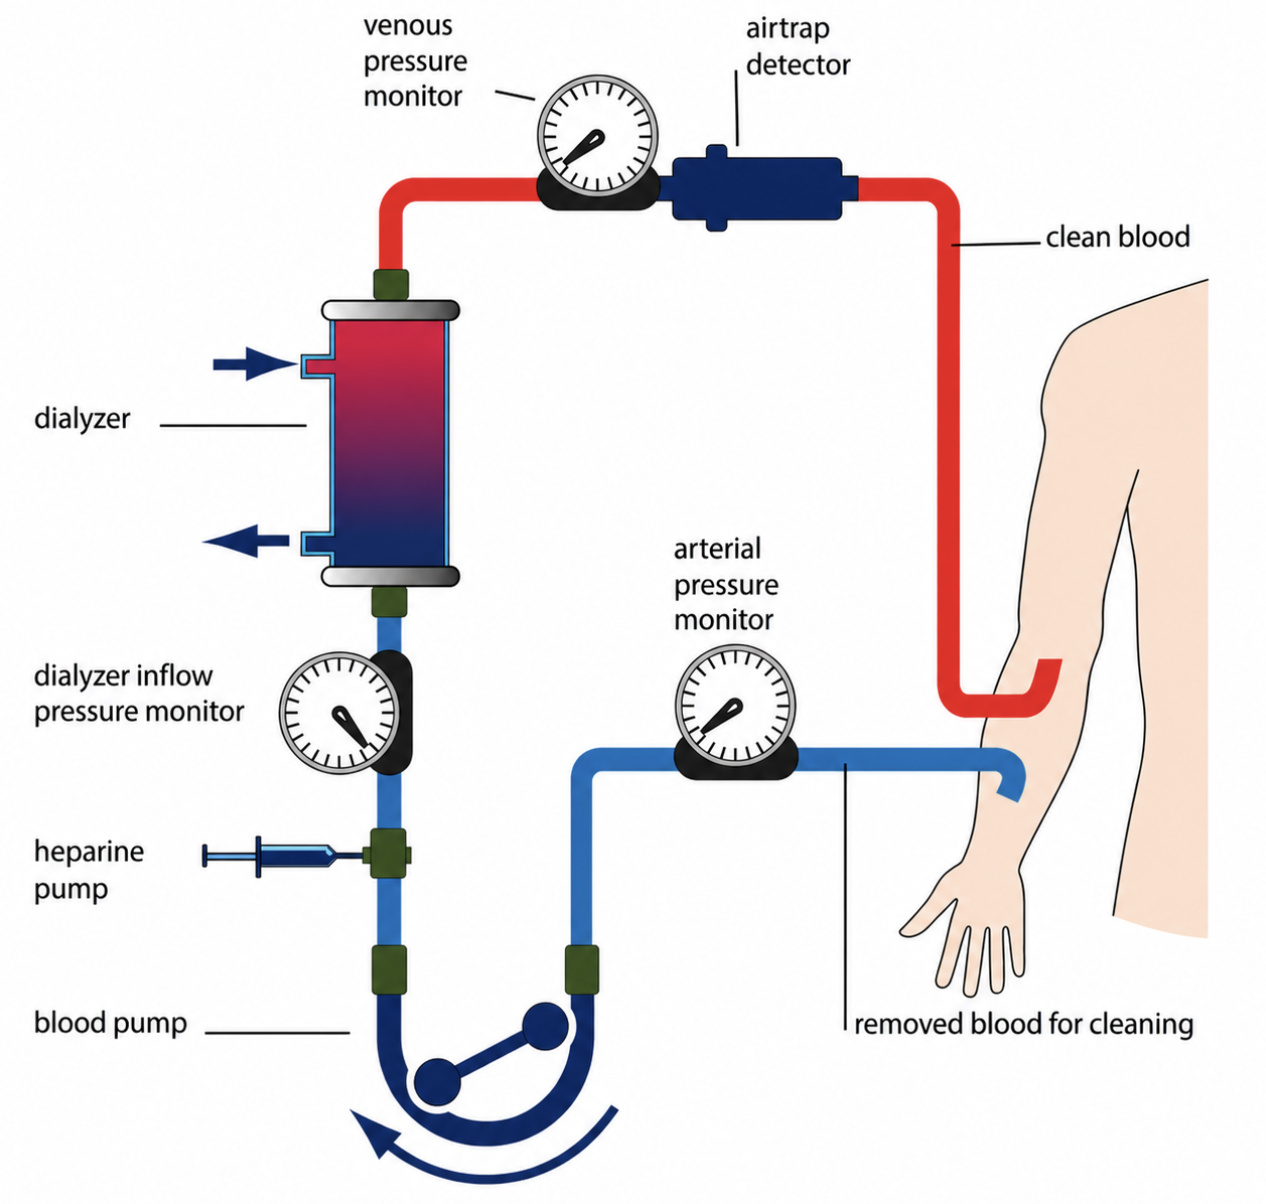
\includegraphics[width=0.60\linewidth]{op989.png}
    \caption{Blood flow through a hemodialysis circuit from the patient, through the dialyzer, and back. \cite{azar_vascular_2013}} 
    \label{fig:placeholder}
\end{figure}


\vspace{-0.3cm}

In this project, hemodialysis is studied as a mass transfer process. Blood flows on one side of a hollow fiber membrane while dialysate flows on the other side, creating a concentration difference that drives urea from the blood into the dialysate\cite{sinha_computational_2025}. The main goal of this project is to determine the membrane surface area required to reduce the urea concentration in the blood from its inlet value to the desired outlet value.

The analysis applies key mass transfer concepts, including Fick’s law, diffusion through a membrane, concentration driving force, and convective mass transfer. Hemodialysis provides a practical example of how transport principles can be used to design biomedical equipment. By calculating the required hollow fiber membrane area and estimating the associated cost, this project connects fundamental mass transfer theory to a real medical device that directly supports patient health.

\section{Methodology}

\subsection{System Description}


The system analyzed in this project is a hollow fiber hemodialysis unit used to remove urea from blood. Hemodialysis is modeled as a membrane separation process in which blood and dialysate flow on opposite sides of a semipermeable membrane\cite{klahan_numerical_2024}. The membrane acts as a selective barrier, allowing small solutes such as urea to diffuse through while retaining larger blood components such as red blood cells and proteins\cite{sinha_computational_2025}.

Contaminated blood enters the dialyzer and flows through the inside of many hollow fibers, which provide the surface area needed for separation. Fresh dialysate flows around the outside of the fibers on the shell side. The two streams move in a counter-current arrangement, as shown in Figure 2, helping maintain the concentration driving force for urea transfer along the length of the dialyzer\cite{sinha_computational_2025}. 


\begin{figure}[H]
    \centering
    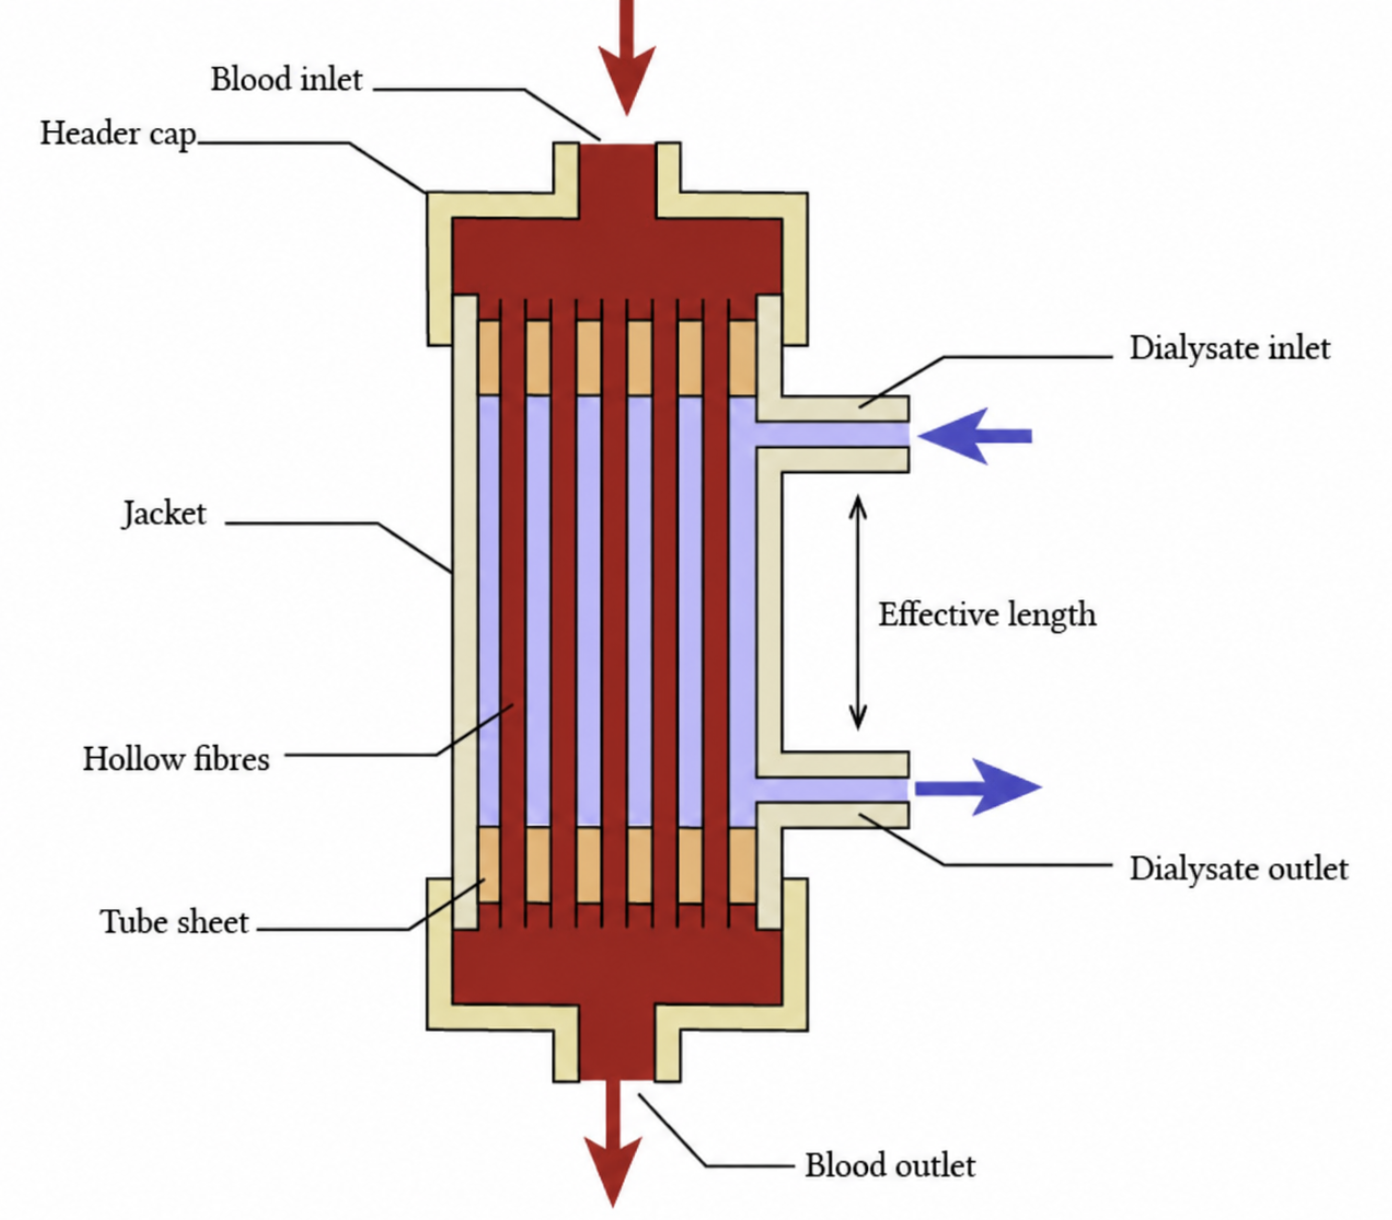
\includegraphics[width=0.5\linewidth]{op88.png}
    \caption{Counter-current flow in a hollow fiber dialyzer, with blood flowing through the fiber lumen and dialysate flowing through the shell side. \cite{yartsev_physical_nodate}}
    \label{fig:placeholder}
\end{figure}



\vspace{-0.5cm}


Urea removal occurs because the urea concentration in the incoming blood is higher than in the fresh dialysate. As a result, urea diffuses from the blood side, through the hollow fiber membrane wall, and into the dialysate. The cleaned blood exits the dialyzer and is returned to the patient, while the spent dialysate leaves carrying the removed urea\cite{sinha_computational_2025}. Figure 3 shows a cross-sectional view of a single hollow fiber, illustrating how urea selectively diffuses through the membrane wall while larger components remain in the blood. 

\begin{figure}[H]
    \centering
    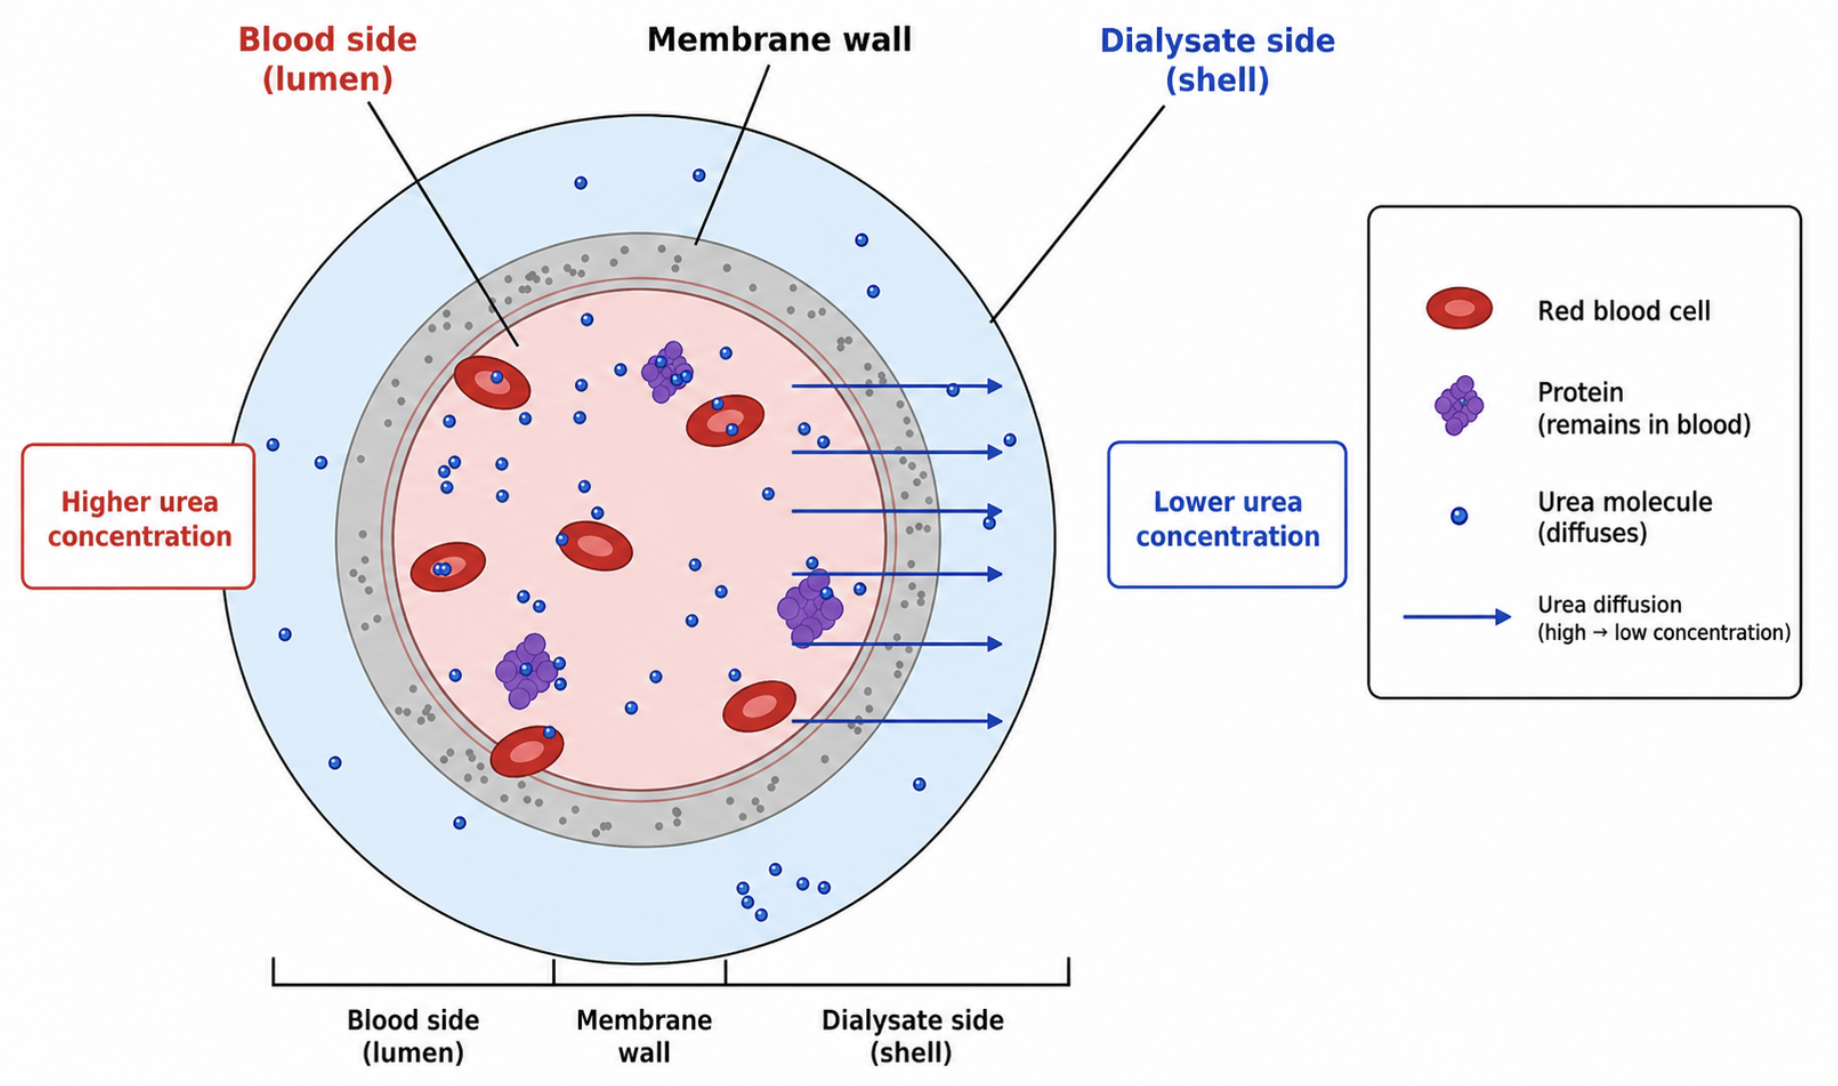
\includegraphics[width=0.75\linewidth]{IKK90.png}
   \captionsetup{justification=centering}
\caption{Cross-sectional hollow fiber membrane showing urea diffusion from blood to dialysate.}
\label{fig:hollow-fiber-cross-section}
\end{figure}


\vspace{-0.2cm}



The hollow fiber configuration provides a large membrane surface area in a compact volume. The dialyzer contains many narrow fibers bundled together, with blood flowing inside each fiber and dialysate flowing outside the fiber. Since the total membrane area depends on the number of fibers, fiber diameter, and fiber length, the system geometry is directly connected to the required membrane area calculation\cite{sinha_computational_2025}.

For this project, the dialyzer is modeled as a steady-state mass transfer device. The main objective is to determine the membrane surface area required to reduce the blood urea concentration from the inlet value to the desired outlet value.

\subsection{Governing Equations}
% https://chatgpt.com/share/69ed3224-f778-83ea-baec-31b13d49cfd5


\subsubsection{Urea Mass Balance Across the Dialyzer}

\begin{equation}
Q_b C_{b,i} + Q_d C_{d,i }= Q_b C_{b,o} + Q_d C_{d,o}
\end{equation}

At steady state, with no urea generation or accumulation inside the dialyzer, this is the total urea balance


\subsubsection{Urea Transport Rate}

The blood-side urea removal rate is:

\vspace{-1cm}

\begin{equation}
\dot{n}_A = Q_b(C_{b,i}-C_{b,o})
\end{equation}

The dialysate-side urea gain is:

\vspace{-1cm}

\begin{equation}
\dot{n}_A = Q_d(C_{d,o}-C_{d,i})
\end{equation}





\vspace{-0.2cm}
\subsubsection{Dialysate outlet concentration}
    
\vspace{0.3cm}

    \begin{equation}
     C_{d,o} = \frac{Q_b}{Q_d}(C_{b,i}-C_{b,o})       
    \end{equation}
    
The spent dialysate concentration depends on the amount of urea removed
from the blood and the dialysate flow rate. This form assumes the fresh
dialysate enters with negligible urea concentration.

\subsubsection{Fick's Law of Diffusion Through the Membrane}

\vspace{0.3cm}

\begin{equation}
    J_A =
    \frac{D_{\text{Ae}}}{\delta_m}
    (C_{A,b}-C_{A,d})
\end{equation}

\vspace{-0.2cm}

The urea flux increases with effective diffusivity and concentration
difference, and decreases as membrane thickness increases.


\subsubsection{Effective Diffusivity}

\vspace{0.1cm}

\begin{equation}
    D_{\text{Ae}} = \varepsilon D_{AB}
\end{equation}

\vspace{-0.3cm}

The effective diffusivity accounts for the fact that only the open pore
volume of the membrane is available for urea diffusion.

\vspace{-0.2cm}



\subsubsection{Overall Mass Transfer Resistance}


\begin{equation}
    \frac{1}{K_o} = \frac{1}{k_b} + \frac{\delta_m}{D_{\text{Ae}}} + \frac{1}{k_d}
    \end{equation}

The overall resistance includes the blood-side film, membrane layer, and dialysate-side film. A larger resistance lowers the overall mass-transfer coefficient.

\subsubsection{Log-Mean Concentration Difference}

\vspace{0.1cm}

\begin{equation}
    \Delta C_{\text{lm}} =
    \frac{\Delta C_1-\Delta C_2}
    {\ln\left(\frac{\Delta C_1}{\Delta C_2}\right)}
\end{equation}

\vspace{-0.5cm}

\begin{equation}
    \Delta C_1 = C_{b,i}-C_{d,o}
\end{equation}

\vspace{-0.5cm}

\begin{equation}
    \Delta C_2 = C_{b,o}-C_{d,i}
\end{equation}

The log-mean concentration difference represents the average driving force for counter-current urea transfer along the dialyzer. The log-mean concentration difference represents the average driving force for counter-current urea transfer along the dialyzer.


\subsubsection{Overall Membrane Mass Transfer}

\vspace{0.1cm}

\begin{equation}
    \dot{n}_A = K_o \cdot A_m \Delta C_{\text{lm}}
\end{equation}

The total urea removal rate depends on the overall mass-transfer coefficient,
available membrane area, and average concentration driving force.

   
\subsubsection{Membrane Surface Area}

\vspace{0.1cm}

\begin{equation}
    A_m =
    \frac{Q_b(C_{b,i}-C_{b,o})}
    {K_o\Delta C_{\text{lm}}}
\end{equation}

\vspace{-0.35cm}

The required area increases when more urea must be removed and decreases
when mass transfer is stronger or the concentration driving force is larger.

\subsection{Assumptions}

\begin{enumerate}
\item The dialyzer operates at steady state with no urea accumulation.

\item Blood and dialysate flow rates remain constant along the dialyzer length.

\item Blood and dialysate flow counter-currently, maintaining a concentration driving force and allowing use of a log-mean concentration difference.

\item The inlet dialysate urea concentration is negligible:
\vspace{-1em}
\[
C_{d,i} \approx 0
\]
\vspace{-4em}
\item The dialyzer operates isothermally at the given operating temperature:
\vspace{-1em}
\[
T = 37.4^\circ C
\]
\vspace{-4em}

\item The dialysate has the same physical properties as water at the operating temperature.

\item Blood is treated as a homogeneous liquid with bulk-average density and viscosity. Blood cells and plasma are not modeled separately.

\item Both streams are well mixed radially. Urea concentrations vary only along the axial length of the dialyzer.

\item The membrane thickness is much smaller than the fiber diameter. Diffusion through the membrane is approximated as one-dimensional diffusion through a flat slab.

\item Urea transport through the membrane follows Fick's Law, driven by the blood-to-dialysate concentration difference.

\item Pressure-driven ultrafiltration is neglected. Urea removal occurs by diffusion only.

\item The membrane void fraction reduces the effective diffusivity of urea:

\vspace{-2em}

\[
D_{\text{Ae}} = \varepsilon \, D_{AB} % , \qquad \varepsilon = 0.2
\]

\vspace{-2em}

\item Mass-transfer resistance is modeled as three resistances in series:

\vspace{-1em}

\[
\frac{1}{K_o} = \frac{1}{k_b} + \frac{\delta_m}{D_{\text{Ae}}} + \frac{1}{k_d}
\]


\item Blood-side and dialysate-side mass-transfer resistances are assumed to be negligible; therefore, membrane resistance dominates.

\vspace{-0.8cm}

\[
\frac{1}{K_o}=\frac{\delta_m}{D_{Ae}}
\]


\vspace{-0.1cm}


\item The full hollow-fiber membrane surface area is assumed to be active and available for urea diffusion.



\end{enumerate}



Overall, these assumptions are reasonable for a preliminary hemodialysis design because they simplify the system enough to estimate the required membrane area. The main limitation is that blood-side and dialysate-side mass-transfer resistances are neglected, so the calculated area may be lower than what would be required in a real dialyzer.

\subsection{Given Parameters}

\vspace{-0.3cm}
\subsubsection{Flow Rate and Concentration Data}

\vspace{-0.2cm}
\begin{itemize}
    \setlength\itemsep{-0.15cm}

    \item Initial urea concentration in bloodstream: 
    \(C_{b,i} = 2000 \ \text{mg/L} = 2.000 \ \text{kg/m}^3\)

    \item Target urea concentration after treatment: 
    \(C_{b,o} = 600 \ \text{mg/L} = 0.600 \ \text{kg/m}^3\)

    \item Blood volumetric flow rate: 
    \(Q_b = 1000 \ \text{mL/min} = 1.000 \times 10^{-3} \ \text{m}^3/\text{min}
    = 1.667 \times 10^{-5} \ \text{m}^3/\text{s}\)

    \item Dialysate volumetric flow rate: 
    \(Q_d = 2400 \ \text{mL/min} = 2.400 \times 10^{-3} \ \text{m}^3/\text{min}
    = 4.000 \times 10^{-5} \ \text{m}^3/\text{s}\)

    \item Dialysate linear velocity: 
    \(v_d = 0.2 \ \text{m/s}\)

    \item Blood linear velocity: 
    \(v_b = \dfrac{v_d Q_b}{2Q_d}
    = \dfrac{(0.2)(1000)}{2(2400)}
    = 0.0417 \ \text{m/s}\)
\end{itemize}

\vspace{-0.4cm}
\subsubsection{Dialyzer Design Specifications}

\vspace{-0.2cm}
\begin{itemize}
    \setlength\itemsep{-0.15cm}

    \item Operating temperature: 
    \(T = 37.4^\circ \text{C} = 310.55 \ \text{K}\)

    \item Fiber length: 
    \(L = 20 \ \text{cm} = 0.200 \ \text{m}\)

    \item Membrane thickness: 
    \(\delta_m = 25 \ \mu\text{m} = 25 \times 10^{-6} \ \text{m}
    = 2.50 \times 10^{-5} \ \text{m}\)

    \item Open void fraction of membrane: 
    \(\varepsilon = 0.2\)

    \item Diffusivity of urea in water at \(26.7^\circ \text{C}\): 
    \(D_{AB,26.7^\circ\text{C}} = 1.44 \times 10^{-9} \ \text{m}^2/\text{s}\)
\end{itemize}

\vspace{-0.4cm}
\subsubsection{Blood and Plasma Properties}

\vspace{-0.2cm}
\begin{itemize}
    \setlength\itemsep{-0.15cm}

    \item Blood cell volume fraction: \(45\% = 0.45\)

    \item Plasma volume fraction: \(55\% = 0.55\)

    \item Blood density: 
    \(\rho_b = 990 \ \text{kg/m}^3\)

    \item Blood viscosity: 
    \(\mu_b = 3.0 \ \text{cP} = 3.0 \times 10^{-3} \ \text{Pa}\cdot\text{s}\)

    \item Plasma composition: greater than \(90\%\) water

    \item Protein concentration in plasma: 
    \(C_{\text{protein}} \approx 75 \ \text{g/L} = 75 \ \text{kg/m}^3\)

    \item Fraction of urea bound with protein: \(30\% = 0.30\)

    \item Average molecular weight of protein: 
    \(MW_{\text{protein}} = 100{,}000 \ \dfrac{\text{kg mass}}{\text{kg mol}}\)
\end{itemize}




\section{Results and Discussion}

Table~\ref{tab:calculated_parameters} summarizes the main calculated parameters used to size the hollow fiber hemodialysis membrane. Detailed unit conversions and intermediate calculations are provided in Appendix A.

\begin{table}[h!]
\centering
\caption{Summary of calculated parameters for the hemodialysis membrane design.}
\label{tab:calculated_parameters}



\renewcommand{\arraystretch}{1.35}

\begin{tabular}{l @{\hspace{0.6cm}} l @{\hspace{0.6cm}} l @{\hspace{0.6cm}} l}
\hline
\textbf{Parameter} & \textbf{Symbol} & \textbf{Value} & \textbf{Units} \\
\hline
Dialysate outlet urea concentration & $C_{d,o}$ & 583.3 & mg/L \\
Temperature-corrected urea diffusivity & $D_{AB,T}$ & $1.87 \times 10^{-9}$ & m$^2$/s \\
Effective membrane diffusivity & $D_{Ae}$ & $3.74 \times 10^{-10}$ & m$^2$/s \\
Overall mass transfer coefficient & $K_o$ & $1.50 \times 10^{-5}$ & m/s \\
Concentration difference at inlet end & $\Delta C_1$ & 1416.7 & mg/L \\
Concentration difference at outlet end & $\Delta C_2$ & 600 & mg/L \\
Log-mean concentration difference & $\Delta C_{lm}$ & 951 & mg/L \\
Urea removal rate & $\dot{m}_A$ & 1400 & mg/min \\
Required membrane surface area & $A_m$ & 1.64 & m$^2$ \\
Number of hollow fibers & $N_f$ & $1.45 \times 10^{4}$ & fibers \\
Estimated membrane cost & -- & 24.60 &  \$ \\

\end{tabular}

\renewcommand{\arraystretch}{2.0}
\end{table}



Using the modeling approach and governing equations described above, key transport parameters and design values for the hemodialysis system were determined. The calculated dialysate outlet concentration, effective diffusivity, overall mass transfer coefficient, and log-mean concentration difference are summarized through the intermediate steps, leading to a required membrane surface area of $1.64 \ \text{m}^2$ and an estimated $1.45 \times 10^4$ hollow fibers. These values were obtained using steady-state mass balances, diffusion relations, and a resistance-based mass transfer model.

\vspace{0.3cm}

The calculated dialysate outlet concentration was $583.3 \ \text{mg/L}$, indicating that a significant portion of urea is transferred from the blood to the dialysate. This result reflects the effect of the higher blood-side concentration relative to the fresh dialysate inlet, which was assumed to be negligible. The relatively high outlet concentration of the dialysate confirms that the system is effectively using the concentration gradient, while still maintaining enough driving force for diffusion along the dialyzer length.

\vspace{0.3cm}


The temperature adjusted diffusivity was determined to be $1.87 \times 10^{-9} \ \text{m}^2/\text{s}$, which increased from the reference value due to the higher operating temperature. After accounting for the membrane porosity, the effective diffusivity was reduced to $3.74 \times 10^{-10} \ \text{m}^2/\text{s}$, demonstrating that only a fraction of the membrane volume contributes to transport. This reduction directly impacts the overall system performance, as it lowers the mass transfer coefficient and increases the membrane area required to achieve the desired separation.

\vspace{0.3cm}


The overall mass transfer coefficient was calculated as $1.50 \times 10^{-5} \ \text{m/s}$, assuming that membrane resistance dominates and that the blood-side and dialysate-side film resistances are negligible. This assumption simplifies the analysis and highlights the importance of membrane properties such as thickness and porosity. However, in practice, boundary layer resistances would contribute to the overall resistance, meaning that the actual mass transfer coefficient may be lower than predicted, resulting in a larger required membrane area.

\vspace{0.3cm}


The concentration driving force was evaluated using the log-mean concentration difference, which was calculated to be approximately $951 \ \text{mg/L}$. The difference between the inlet and outlet concentration differences ($\Delta C_1 = 1416.7 \ \text{mg/L}$ and $\Delta C_2 = 600 \ \text{mg/L}$) shows that while the driving force decreases along the length, it does not reach a very low value, allowing diffusion to occur continuously.

\vspace{0.3cm}


The calculated urea removal rate was $1400 \ \text{mg/min}$, which directly depends on the blood flow rate and the concentration drop across the system. Using this removal rate along with the calculated mass transfer coefficient and driving force, the required membrane area was determined to be $1.64 \ \text{m}^2$. The corresponding number of fibers, approximately $1.45 \times 10^4$, reflects the advantage of hollow fiber designs.

\vspace{0.3cm}


The results are sensitive to several design and operating parameters. A decrease in membrane thickness or an increase in effective diffusivity would increase the mass transfer coefficient and reduce the required membrane area. Increasing the dialysate flow rate would reduce the dialysate outlet concentration, increasing the concentration driving force and improving overall performance. Lower flow rates or reduced diffusivity would decrease transport efficiency and require a larger membrane area.

\vspace{0.3cm}


Several assumptions were made in this analysis that can impact the accuracy of the results. The system was assumed to operate at steady state with constant flow rates and negligible dialysate inlet concentration. Urea transport was modeled as purely diffusive, neglecting any contribution from pressure-driven ultrafiltration. Additionally, blood was treated as a homogeneous fluid, and the resistances associated with boundary layers were neglected.

\vspace{0.3cm}


The estimated membrane cost was approximately \$24.60, based on membrane area. This value is lower than what would be expected for a dialysis system, as it does not include any costs related to manufacturing or operational costs.

\vspace{0.3cm}


Overall, the results demonstrate that urea removal in a hemodialysis system is governed by the combined effects of concentration driving force, membrane resistance, and flow conditions.

\vspace{0.3cm}



\section{Conclusion}

The goal of this analysis was to determine the membrane surface area required for a hemodialysis system to achieve a specified reduction in blood urea concentration using mass transfer principles and a diffusion-based transport model. By applying steady-state mass balances, resistance-based transport relations, and log-mean concentration difference analysis, key system parameters including the overall mass transfer coefficient, effective diffusivity, and concentration driving force were evaluated.

\vspace{0.3cm}


The calculation analysis determined that a membrane surface area of approximately $1.64 \ \text{m}^2$ is required to achieve the desired urea removal, corresponding to about $1.45 \times 10^4$ hollow fibers. These results indicate that a large membrane area is necessary, confirming that urea removal in hemodialysis is a diffusion limited process. The use of a hollow fiber configuration is appropriate, since it allows a large surface area to be implemented within a small device that can maintain effective mass transfer.

\vspace{0.3cm}


Hemodialysis performance can be improved by increasing the membrane surface area, which enhances the available area for mass transfer and allows more urea to diffuse across the membrane. Additionally, increasing the dialysate flow rate helps maintain a higher concentration gradient between the blood and dialysate streams, thereby improving the overall driving force for diffusion. Another important factor is the membrane void fraction (porosity); increasing the porosity increases the effective diffusivity within the membrane, allowing solutes to pass through more easily. However, this must be done carefully while considering protein size. 






\newpage





\bibliographystyle{ieeetr}
\bibliography{references}

\newpage
\section*{Appendix}













\subsection*{Calculations}

\subsubsection{Dialysate Outlet Concentration, $C_{d,o}$}

Using the total urea mass balance,
\[
    Q_b(C_{b,i}-C_{b,o}) = Q_d(C_{d,o}-C_{d,i})
\]

Since fresh dialysate enters with negligible urea concentration, $C_{d,i}=0$. Solving for $C_{d,o}$:
\[
    C_{d,o} = \frac{Q_b}{Q_d}(C_{b,i}-C_{b,o})
    = \frac{1000}{2400}(2000-600)
\]

\[
    \boxed{C_{d,o}=583.3 \ \text{mg/L}}
\]

\subsubsection{Temperature-Corrected Urea Diffusivity, $D_{AB,T}$}

The diffusivity is corrected using:
\[
    D_{AB,T}
    = D_{AB,ref}
    \left(\frac{T}{T_{ref}}\right)
    \left(\frac{\mu_{ref}}{\mu_T}\right)
\]

The temperatures are converted to Kelvin:
\[
    T_{ref}=26.7+273.15=299.85 \ \text{K},
    \qquad
    T=37.4+273.15=310.55 \ \text{K}
\]

Substituting values:
\[
    D_{AB,T}
    = (1.44 \times 10^{-9})
    \left(\frac{310.55}{299.85}\right)
    \left(\frac{878.263 \times 10^{-6}}{699.037 \times 10^{-6}}\right)
\]

\[
    D_{AB,T}
    = (1.44 \times 10^{-9})(1.0357)(1.2564)
\]

\[
    \boxed{D_{AB,T}=1.87 \times 10^{-9} \ \text{m}^2/\text{s}}
\]

\subsubsection{Effective Diffusivity, $D_{Ae}$}

The effective diffusivity through the membrane is:
\[
    D_{Ae} = \varepsilon D_{AB,T}
    = (0.20)(1.87 \times 10^{-9})
\]

\[
    \boxed{D_{Ae}=3.74 \times 10^{-10} \ \text{m}^2/\text{s}}
\]

\subsubsection{Overall Mass Transfer Coefficient, $K_o$}

Assuming membrane resistance dominates:
\[
    K_o \approx \frac{D_{Ae}}{\delta_m}
    = \frac{3.74 \times 10^{-10}}{25 \times 10^{-6}}
\]

\[
    \boxed{K_o=1.50 \times 10^{-5} \ \text{m/s}}
\]

\subsubsection{Concentration Differences, $\Delta C_1$ and $\Delta C_2$}

For counter-current flow:
\[
    \Delta C_1 = C_{b,i}-C_{d,o},
    \qquad
    \Delta C_2 = C_{b,o}-C_{d,i}
\]

Since $C_{d,i}\approx 0$:
\[
    \Delta C_1 = 2000-583.3 = 1416.7 \ \text{mg/L}
\]

\[
    \Delta C_2 = 600-0 = 600 \ \text{mg/L}
\]

\[
    \boxed{\Delta C_1=1416.7 \ \text{mg/L}},
    \qquad
    \boxed{\Delta C_2=600 \ \text{mg/L}}
\]

\subsubsection{Log-Mean Concentration Difference, $\Delta C_{lm}$}

The log-mean concentration difference is:
\[
    \Delta C_{lm}
    =
    \frac{\Delta C_1-\Delta C_2}
    {\ln\left(\frac{\Delta C_1}{\Delta C_2}\right)}
\]

Using $\Delta C_1=1416.7 \ \text{mg/L}$ and $\Delta C_2=600 \ \text{mg/L}$:
\[
    \Delta C_{lm}
    =
    \frac{1416.7-600}
    {\ln\left(\frac{1416.7}{600}\right)}
    =
    \frac{816.7}{0.859}
\]

\[
    \boxed{\Delta C_{lm} \approx 951 \ \text{mg/L}}
\]

\subsubsection{Urea Removal Rate, $\dot{m}_A$}

The mass removal rate is:
\[
    \dot{m}_A = Q_b(C_{b,i}-C_{b,o})
    = (1.0)(2000-600)
    = 1400 \ \text{mg/min}
\]

\[
    \boxed{\dot{m}_A = 1400 \ \text{mg/min}}
\]

\subsubsection{Required Membrane Surface Area, $A_m$}

The required membrane area is:
\[
    A_m =
    \frac{Q_b(C_{b,i}-C_{b,o})}
    {K_o \Delta C_{lm}}
\]

Using $Q_b=1.0 \ \text{L/min}=1.667 \times 10^{-5} \ \text{m}^3/\text{s}$:
\[
    A_m
    =
    \frac{(1.667 \times 10^{-5})(1400)}
    {(1.50 \times 10^{-5})(951)}
    =
    \frac{2.334 \times 10^{-2}}
    {1.4265 \times 10^{-2}}
\]

\[
    \boxed{A_m \approx 1.64 \ \text{m}^2}
\]

\subsubsection{Number of Hollow Fibers, $N_f$}

The membrane area is related to hollow fiber geometry by:
\[
    A_m = N_f \pi d_f L
\]

Solving for $N_f$:
\[
    N_f = \frac{A_m}{\pi d_f L}
\]

Using $A_m=1.64 \ \text{m}^2$, $d_f=180 \ \mu\text{m} \cite{perez-garcia_dializador_2018} = 1.80 \times 10^{-4} \ \text{m}$, and $L=0.20 \ \text{m}$:
\[
    N_f
    =
    \frac{1.64}
    {\pi(1.80 \times 10^{-4})(0.20)}
    =
    \frac{1.64}{1.131 \times 10^{-4}}
\]

\[
    \boxed{N_f \approx 1.45 \times 10^4 \ \text{fibers}}
\]

\subsubsection{Membrane Cost}

The total membrane cost is:
\[
    \text{Cost}
    =
    A_m \left(\frac{\$}{\text{m}^2}\right)
\]

Using $A_m=1.64 \ \text{m}^2$ and a membrane cost of $15 \ \$/\text{m}^2$ \cite{yehl_single-use_2020}:
\[
    \text{Cost} = 1.64(15)
\]

\[
    \boxed{\text{Cost} \approx \$24.60}
\]


\end{document}
